\section{Implications for the study and optimization of \acs{WCA}}\label{sec:implications}
\todo[inline]{Implications for \ac{WCA} footprint.}
\todo[inline]{Two subsections (simulation and real system.)}
\todo[inline]{Leave it for now.}
% \todo[inline]{Introduction to this section?}

\subsection{Application lifetimes}

We begin by studying the implications of such a model on the estimation of application lifetimes.
In the context of \ac{WCA}, we will understand \emph{application lifetime} as the time it takes a user to complete a specified task.
This is an important metric for \ac{WCA} optimization, as it directly relates to system resource utilization and contention, and to energy consumption.

In order to illustrate the consequences of using a less realistic model which does not take into account higher order effects, we introduce here a reference model to which we will compare our more realistic models.
This new model represents a first-order approximation to empirical execution time modeling, and consist simply of an \ac{exGaussian} distribution fitted to all execution time samples collected for \textcite{olguinmunoz:impact2021}.
This distribution is then randomly sampled at runtime to obtain execution times for each step, without any sort of adjustment to the current state of the system.

We start by studying application lifetimes in a controlled, ideal setup by using the timing models to generate execution times for sequences of \num{100} steps subject to constant \acp{TTF}.
These runs are completely simulated and no sampling of video frames is performed; for each step, we simply feed the models a predefined \ac{TTF} and record the generated execution time.
We use the combination of \acp{TTF} and execution times to calculate theoretical step duration times and subsequent total application lifetimes.
This is done for \num{25} linearly distributed \acp{TTF} in the \SIrange[]{0}{5}{\second} range; \num{45} independent repetitions for each combination of model configuration and \ac{TTF}.

\begin{figure}
    \centering
    \begin{subfigure}[]{\columnwidth}
        \centering
        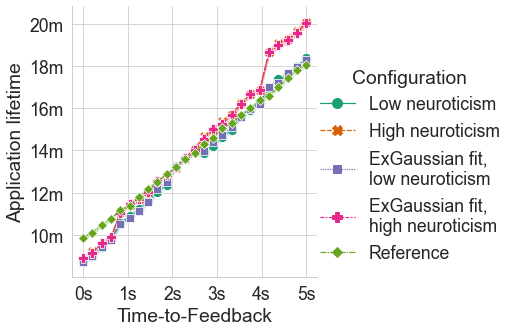
\includegraphics[width=\textwidth]{figs/new_model/lifetime_all_ttfs.png}
        \caption{%
            Evolution of mean application lifetimes as \acp{TTF} increase.
            Error bars indicate \SI{95}{\percent} \acp{CI}.
        }
    \end{subfigure}
    \begin{subfigure}[]{\columnwidth}
        \centering
        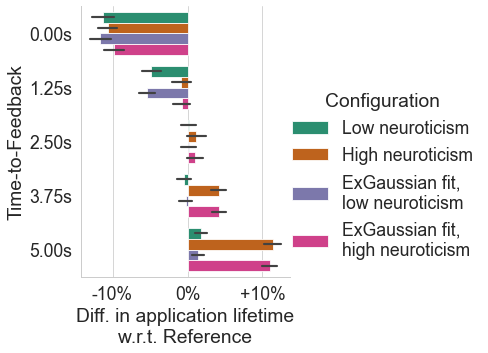
\includegraphics[width=\textwidth]{figs/new_model/lifetime_diff.png}
        \caption{%
            Percentage difference in mean application lifetimes with respect to the reference model at select \acp{TTF}.
            Error bars indicate the \SI{95}{\percent} \acp{CI}, calculated using a two-sided T-test.
        }
    \end{subfigure}
    \caption{\acl{TTF} versus application lifetime.}\label{fig:lifetimes}
\end{figure}

The results of this investigation are presented in \cref{fig:lifetimes}.
Compared to the reference model, our realistic model is, on average, roughly \SI{11}{\percent} faster when subject to low \acp{TTF}.
At higher \acp{TTF}, the behavior of the model depends on its level of normalized neuroticism.
At low neuroticism, the behavior of the realistic model results in total task durations that are basically indistinguishable from the reference model.
However, at high neuroticism, the model once again results in a considerable difference in total task duration with respect to the reference --- this time extending durations by \textasciitilde\SI{11}{\percent} on average.

\begin{figure}
    \centering
    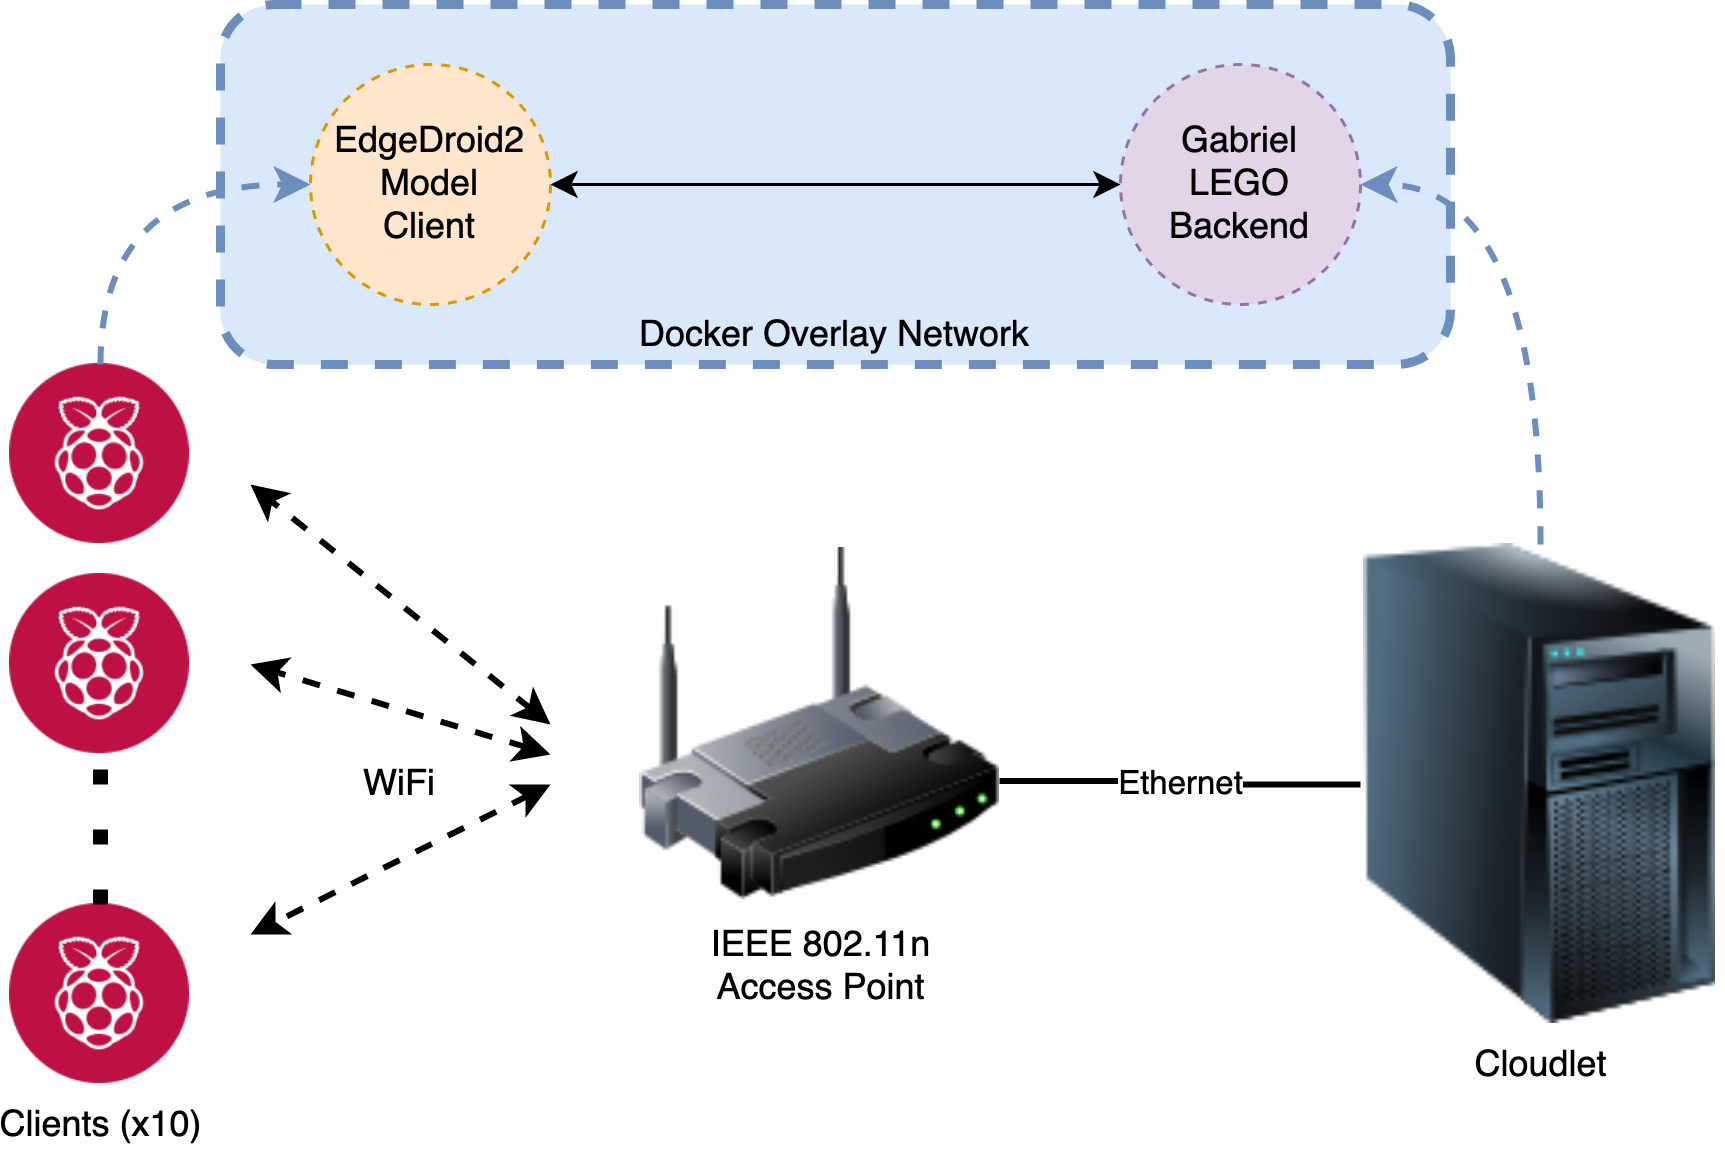
\includegraphics[width=\columnwidth]{figs/EdgeDroid2ExperimentalSetup.png}
    \caption{%
        Experimental setup used to study the implications of the realistic models of human behavior for \ac{WCA}.
        We deploy containerized instances of the client-server loop running the models on a testbed consisting of \num{10} Raspberry Pi clients connected to a cloudlet over a \acs*{COTS} \acs{IEEE} \num{802.11}b/g access point.
    }\label{fig:expsetup}
\end{figure}

Next we study the effects of first- versus second-order models in a more realistic setting.
The models, reference and realistic, are deployed on the Raspberry Pi clients of the testbed depicted in \cref{fig:expsetup}.
For this, the timing models and frame generator are integrated into a custom Python3 client for the Gabriel \ac{WCA} platform~\cite{Chen2018application}, which are then paired with real instances of Gabriel deployed on the cloudlet.
Clients and cloudlet communicate over an \acs{IEEE} \num{802.11}b/g wireless network.
Our choice of wireless standard is simply motivated by a desire to amplify the potential effects of network congestion.
\todo[inline]{More justification?}

\begin{figure}
    \centering
    \begin{subfigure}[]{\columnwidth}
        \centering
        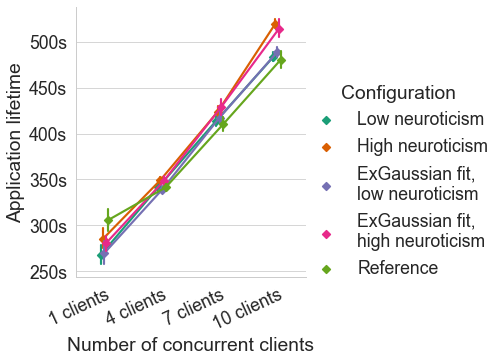
\includegraphics[width=\textwidth]{figs/new_model/lifetime_testbed.png}
        \caption{%
            Mean application lifetimes per testbed configuration.
            Note that due to the low number of samples, means have been calculated using the geometric instead of arithmetic average. 
            Error bars indicate \SI{95}{\percent} \acp{CI}, calculated using bootstrapping.
        }
    \end{subfigure}
    \par\bigskip
    \begin{subtable}{\columnwidth}
        \centering
        \begin{tabular}{lrrrr}
            \toprule
            \# clients & 1 & 4 & 7 & 10 \\
            \ac{RTT} & \SI{0.42}{\second} & \SI{1.12}{\second} & \SI{1.92}{\second} & \SI{2.68}{\second} \\
            \bottomrule
        \end{tabular}
        \caption{Mean measured \aclp{RTT} for each testbed configuration.}
    \end{subtable}
    \par\bigskip
    \begin{subfigure}[]{\columnwidth}
        \centering
        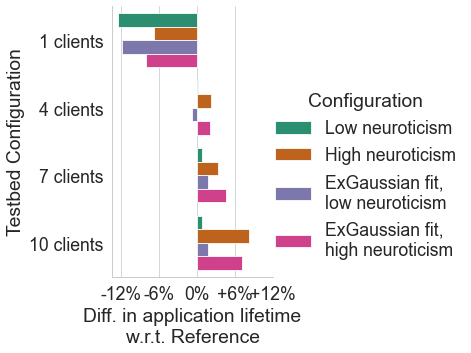
\includegraphics[width=\textwidth]{figs/new_model/lifetime_testbed_diff.png}
        \caption{%
            Percentage difference in mean application lifetimes with respect to the reference model.
            Confidence intervals have been omitted due to the low number of samples and the use of the geometric mean.
        }
    \end{subfigure}
    \caption{Application lifetimes in the realistic scenarios.}\label{fig:testbed_lifetimes}
\end{figure}

We deploy configurations running \num{45}-step versions of the LEGO task described in \textcite{olguinmunoz:impact2021}.
The testbed configurations include setups with \numlist{1;4;7;10} clients.
Due to having only limited time, each combination of testbed and timing model configuration is only repeated \num{10} times.
The results are presented in \cref{fig:testbed_lifetimes}.
Owing to the low number of samples, we opt here for the geometric rather than arithmetic mean to represent our results.
The results are nonetheless clear, and follow the same pattern as the previously discussed results under ideal, controlled circumstances.
With just a single client and mean \ac{RTT} of around \SI{400}{\milli\second}, all parameterizations of the realistic model achieved an average task duration \SIrange{6}{12}{\percent} shorter than the reference.
At \num{10} clients, the results mimic those at higher \acp{TTF} in the ideal controlled setup, with high neuroticism parameterizations reaching \textasciitilde\SI{8}{\percent} longer application lifetimes.

These results highlight the importance of accurate execution time modeling when studying \ac{WCA} application lifetimes.
Not only do we see considerable differences in lifetimes at relatively moderate levels of system congestion, but the sign of these differences depends on the load placed on the system.
Imagine thus a system designer studying resource consumption optimization in a \ac{WCA}.
If they were to employ the reference model for their study on an unimpaired system, it could lead them to significantly underestimate the potential for optimization of resource consumption, leaving performance (and, potentially, monetary) gains on the table.
On the other hand, under heavy load, they would instead underestimate system resource occupation, again leading to performance losses.

\todo[inline]{%
    Ergo we need a second order model. Everything that comes afterwards is only with second order model. Play with RTT.
}


% .as well as an additional setup with \num{10} clients during which an instance of the \emph{iperf3}\footnote{\href{https://iperf.fr/}{https://iperf.fr/}} network load generator is also running on each client.
% The \emph{iperf3} instances each generate \SI{1.5}{Mbps} of upstream \ac{TCP} traffic, further congesting the wireless network.

\subsection{Optimizing for mean number of samples per step}

In~\cite{Wang2019Towards}, \citeauthor{Wang2019Towards} introduce an adaptive sampling scheme for \ac{WCA} intended to reduce the number of samples processed per step while still meeting application responsiveness bounds.
At every sampling instant \( t \), the scheme adapts the sampling rate \( R(t) \) of the system according to the estimated likelihood of the user having finished the step,
following the formula 

\begin{equation}
    R(t) = R_\text{min} + \alpha\left( R_\text{max} - R_\text{min} \right) * CDF(t)
\end{equation}

\( R_\text{max} \) and \( R_\text{min} \) correspond to the maximum and minimum sampling rates of the system, respectively.
\( R_\text{max} \) can directly be assumed to correspond to \( 1 / \text{\ac{RTT}}_\mu \), where \( \text{\ac{RTT}}_\mu \) corresponds to the mean \ac{RTT} of the system.
\( R_\text{min} \) needs to either be calculated according to the latency bounds of the system or specified manually, and \( \alpha \) corresponds to a scaling factor and \( t \) to the time of the current sampling instant with respect to the start of the step.
Finally, \( CDF \) corresponds to the \ac{CDF} of a distribution describing the execution times for the current step; \citeauthor{Wang2019Towards} used a single static Gaussian distribution for all steps in their work.

In the following, we will show the effects of more accurate execution time estimation using our timing models on the performance of this adaptive scheme.
For this, we implement two variants of the adaptive scheme.
The first one corresponds a reference implementation using \citeauthor{Wang2019Towards}'s original design, using a Gaussian distribution fitted to all the execution times collected for~\cite{olguinmunoz:impact2021} for \ac{CDF} calculation.
This variant the same \ac{CDF} for every step.
The second variant instead uses an embedded internal execution time model to keep track of the \acp{TTF} of the system and adjust the distribution of execution times following the state of the timing model.
In other words, in this variant the \ac{CDF} used for instantaneous calculation of the sampling rate \( R \) changes over time according to the state of the execution time model.
For timing model configurations which do not fit a distribution to execution time data, the \ac{CDF} corresponds to the \ac{ECDF} of the selected execution times.

We proceed to set up an experiment where these sampling scheme variants are deployed on identical, simulated, \num{100}-step tasks.
Also included for reference in this experiment is greedy (also known as \emph{zero-wait}) sampling, where samples are taken as fast as possible; a new sample is taken as soon as the result for the previous one has been received.
This is the default sampling strategy used in most existing \ac{WCA} prototypes.
The execution times for each step are generated by a realistic model parameterized with high neuroticism and without any distribution fitting on the data (this timing model is separate from the internal timing models inside the sampling schemes).
We set \( R_\text{min} \) to \SI{0.5}{\hertz} and \( \alpha \) to \num{3.0}.
The \ac{RTT} of the system is set to one of \SIlist[list-final-separator={, or}]{150;300;600}{\milli\second}, constant for all steps of the task.
For each combination of sampling scheme configuration (original adaptive by \textcite{Wang2019Towards}, adaptive with \edgedroid{} model, greedy) and \ac{RTT}, we run \num{100} repetitions of the task for good statistical significance.

\begin{figure*}
    \centering
    \begin{subtable}[t]{.25\textwidth}
        \centering
        \caption{Parameters used for \textcite{Wang2019Towards}'s adaptive sampling scheme.}
        \medskip
        \begin{tabular}{lr}
            \toprule
            \( R_\text{min} \)  & \SI{0.5}{\hertz} \\
            \( \alpha \)        & \num{3.0} \\
            \ac{RTT}            & \SIlist{150;300;600}{\milli\second} \\
            \bottomrule
        \end{tabular}
    \end{subtable}%
    \hspace{.05\textwidth}%
    \begin{subtable}[t]{.65\textwidth}
        \centering
        \caption{Mean number of captured samples per sampling scheme at the three different \acp{RTT}.}
        \medskip
        \begin{tabular}{llrrr}
            \toprule 
            Timing model neuro. & Sampling scheme & \SI{150}{\milli\second} & \SI{300}{\milli\second} & \SI{600}{\milli\second} \\
           \midrule
           \multirow[c]{2}{*}{Low} & Greedy & \num{36.53} & \num{18.88} & \num{10.52} \\
            & Adaptive Gaussian fit & \num{19.97} & \num{10.43} & \num{6.39} \\
           \multirow[c]{2}{*}{High} & Greedy & \num{37.05} & \num{19.04} & \num{10.89} \\
            & Adaptive Gaussian fit & \num{20.29} & \num{10.79} & \num{6.67} \\
            \bottomrule
        \end{tabular}
    \end{subtable}\\
    \bigskip
    \begin{subfigure}[]{\textwidth}
        \centering
        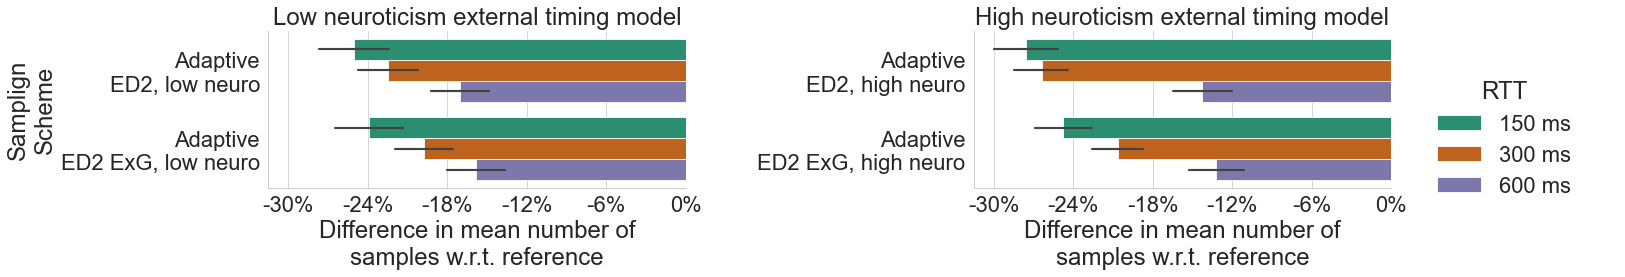
\includegraphics[width=\textwidth]{figs/new_model/diff_sampling_junjue_both.png}
        \caption{%
            Percentage reduction in mean number of captured samples per step (higher is better).
            Error bars indicate the \SI{95}{\percent} \acp{CI}, calculated using a two-sided T-test.
            \todo[inline]{%
                % Vishnu: minimize number of samples.
                I don't like the two plots, I think the message gets diluted and confusing.
                I suggest only keeping one ``ground truth'', high neuroticism.
                Otherwise, every plot and table needs to be duplicated.
            }
        }
    \end{subfigure}
    \caption{%
        Results of parameterizing \textcite{Wang2019Towards}'s adaptive sampling scheme using the realistic timing model.
        \emph{ED2} indicates a sampling scheme using the \edgedroid{} model for \ac{CDF} estimation.
        \emph{HN} and \emph{LN} indicate high or low neuroticism, respectively, and \emph{ExG fit} indicates a timing model which fits an \ac{exGaussian} distribution to the execution time data for each step.
    }\label{fig:samples}
\end{figure*}

The results of this investigation are presented in \cref{fig:samples}
They clearly show the potentially dramatic effects of more accurate execution time estimation when optimizing sampling rates.
When using the realistic model for execution time estimation, the sampling schemes achieve between \SI{14}{\percent} and \textasciitilde\SI{27}{\percent} better average performance, depending on the \edgedroid{} model parameterization and the system \ac{RTT}.
\todo[inline]{Update with new ground truths.}
This is true even for configurations with low neuroticism which do not exactly match the parameterization of the external timing model driving the execution times for the steps, showing thus the importance of even less-accurate approximations.

\subsection{Optimizing for energy consumption}

Energy consumption is another yet unexplored dimension of \ac{WCA} with great opportunities for optimization.
To explore the potential implications of our realistic model of human timings for energy consumption, we will introduce here a novel scheme for sampling in step-based \ac{WCA} systems.

We begin by assuming a given execution time distribution \( \mathcal{T} \), and take the modeling and partial solution approach from recents works on energy efficient sampling in edge-based feedback systems.
In \textcite{ICCperiodic1,TMCperiodic}, the authors model the energy in terms of the expected number of samples $\mathbb{E}[\mathcal{S}]$ and the expected wait time $\mathbb{E}[\mathcal{W}]$ experienced by the user.
The authors then find the optimum periodic sampling interval that minimizes this energy, or equivalently the non-constant parts of this energy termed as \textit{Energy Penalty}.

% In this optimization, the constant parts are excluded as it does not affect the process.
With a value much smaller than the execution time of the event, the \ac{RTT} of the final sample is included in this constant part, which is why $\mathcal{W}$ is computed without it.
Next, in \textcite{secAperiodic}, the author retains the model, removes the constraint of periodicity, and finds the optimum aperiodic sampling instants $\{t_n,\,n=1,2,\dots\}$ that minimize the same energy penalty.

In this work, we use the modeling from~\cite{secAperiodic} to find the optimum aperiodic sampling interval.
However, instead of using their two-step approach to find the solution which includes a recursive solution followed by a bisection algorithm, we develop a novel, approximate, but easier solution to finding the set of the optimum aperiodic sampling intervals.
Furthermore, instead of directly optimizing for energy, we start by noting that an objective metric of a variety of optimization problems that are related to sampling, RTT, responsiveness or wait time present themselves 
% in a format similar to that of the energy, 
as a linear combination between $\mathbb{E}[\mathcal{S}]$ and $\mathbb{E}[\mathcal{W}]$ plus terms independent of the number of samples or wait time.
Let $\mathcal{E}$ correspond to such an objective metric.
Thus,
\begin{alignat}{1}
    \Rightarrow\mathcal{E}&=\alpha\mathbb{E}[\mathcal{S}]+\beta\mathbb{E}[\mathcal{W}]+C,\;\label{eq:epsilon_terminal}
\end{alignat}
\todo[inline]{
Optimization is own section.    
First thing in optimization. Represents a lot of tradeoffs in these systems. For two particular metrics, we discuss solutions of this equations for different optimization purposes. We compare to other approaches. State of the art and offline optimum.
Optimization business should go into own section.}
Here, $\alpha, \beta$ and $C$ are constants which are responsible for modifying the objective function from one metric to another.
For instance, in the modeling used by \textcite{ICCperiodic1,TMCperiodic,secAperiodic}, the chosen characterization results in a metric which is equal to the energy penalty.
The outline of our solution that minimizes \cref{eq:epsilon_terminal} is provided below with the complete mathematical derivation in \cref{appx1}.

\subsubsection{General solution}\label{sec:aprxSol}

Define an instantaneous sampling rate function $r(t)$ which is related to $\{t_n\}$ such that,
\begin{alignat}{1}
{\int_{t_{n-1}}^{t_n}}r(t)\dif t=1,\;\forall n\geq1.\label{rt}
\end{alignat}
For instance, for periodic sampling, the rate function is a constant equal to the sampling frequency. 
% Using this rate function, we rewrite the expected number of samples as
% \begin{alignat}{1}
% \mathbb{E}[\mathcal{S}]&=\int_{t=0}^{\infty}\bigg(\!\int_{x=0}^{t}\!\!\!\!r(x)\,\mathrm{d}x\bigg)f_{\mathcal{T}}(t)\,\mathrm{d}t,\nonumber
% \end{alignat}
% and the approximate the expected wait time as
% \begin{alignat}{1}
% \mathbb{E}[\mathcal{W}]&=\int_{0}^{\infty}\dfrac{1}{2r(t)}f_\mathcal{T}(t)\,\mathrm{d}t.\nonumber
% \end{alignat}
Now, rewriting \cref{eq:epsilon_terminal} in terms of $r(t)$ and minimizing it gives as an optimum rate function $r^*(t)$ as
\begin{alignat}{1}
r^*(t)&=\sqrt{\dfrac{\beta f_\mathcal{T}(t)}{2\alpha\bar{F}_\mathcal{T}(t)}}.\nonumber\\
\intertext{Thus, for a Rayleigh distributed $\mathcal{T}$ with parameter $\sigma$,}
r^*(t)&=\sqrt{\dfrac{\beta t}{2\alpha\sigma^2}}\nonumber\\
% \Rightarrow &\int_{t_n}^{t_{n+1}}\!\!\!\sqrt{\dfrac{\beta t}{2\alpha\sigma^2}}\,\mathrm{d}t=1,\;\forall n\geq1\nonumber\tag{from \eqref{rt}}\\
% \Rightarrow &\;t_{n+1}^{\frac{3}{2}}-t_{n}^{\frac{3}{2}}=3\sigma\!\sqrt{\tfrac{\alpha}{2\beta}}\nonumber\\
\Rightarrow t_n&=\Big(3\sigma\!\sqrt{\tfrac{\alpha}{2\beta}}\Big)^{\frac{2}{3}}n^{\frac{2}{3}}.\label{tn_approx_rayleigh}
\end{alignat}

\subsubsection{Energy minimization}\label{sec:aprxSol_Energy}

With the general solution available, minimizing energy $E$ boils down to finding the appropriate $\alpha$ and $\beta$ that $\mathcal{E}=E$ in \cref{eq:epsilon_terminal}.
For this, we directly take the modeling from~\cite{secAperiodic} with a necessary modification in the assumption of one-way communication in all but the final sample.
With feedback given even to the discarded samples in our model, we have, 
\begin{alignat}{2}
    \mathrm{E}=&\;2\mathcal{S}\tau_cP_c+(\mathcal{T}+\mathcal{W}+\tau_\mathrm{p}+2\tau_\mathrm{c}-2\mathcal{S}\tau_c)P_0\nonumber\\
    % &=s\tau_c(P_c-P_0^{(t)})+wP_0^{(t)}+(\tau+\tau_c+\tau_p) P_0^{(t)}+\tau_cP_c\\
    =&\;2\tau_{\text{c}}(P_{\text{c}} -P_0)\mathcal{S}+\mathcal{W}P_0+(\mathcal{T}+\tau_{\text{p}} +2\tau_{\text{c}}) P_0\nonumber\\
&\Rightarrow \alpha=2\tau_{\text{c}}(P_{\text{c}} -P_0),\text{ and }\beta=P_0.\nonumber
\end{alignat}

\todo[inline]{is communication delay and processing delay defined already?}

\subsubsection{Minimizing number of samples }\label{sec:aprxSol_Energy_samples}

Apart from energy, another common optimization metric is simply the number of samples.
However, an unconstrained optimization of the number of samples is trivial and meaningless as the solution points to a single sample at $t\!\rightarrow\!\infty$, which also takes the wait time to infinity.
We look at the constrained optimization of the expected number of samples with an upper bound $w_0$ for the expected wait.
That is, $\mathbb{E}[\mathcal{W}]\!\leq\!w_0$. We show in \cref{appx1} that the appropriate $\alpha$ and $\beta$ for this problem satisfies the condition
\begin{alignat}{1}
\frac{\alpha}{\beta}=\frac{2\sqrt{2}\,w_0^2}{(\mathlarger{\Gamma}(\tfrac{3}{4}))^2\,\sigma}\approx1.9\frac{w_0^2}{\sigma},\nonumber
\end{alignat}
where, $\mathlarger{\Gamma}(x)$ is the Gamma function.


\subsubsection{Evaluating the impact of the realistic timing model on the energy-optimal sampling scheme}

\begin{figure*}
    \centering
    \begin{subfigure}[t]{\textwidth}
        \centering
        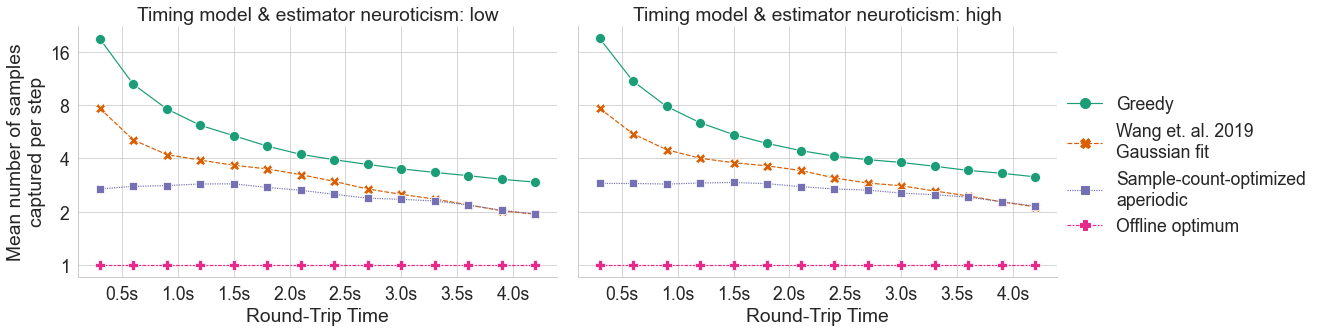
\includegraphics[width=\textwidth]{figs/new_model/sampling_optimization.png}
        \caption{\todo[inline]{Note logarithmic yscale.}}
    \end{subfigure}\\
    \medskip
    \begin{subfigure}[t]{\textwidth}
        \centering
        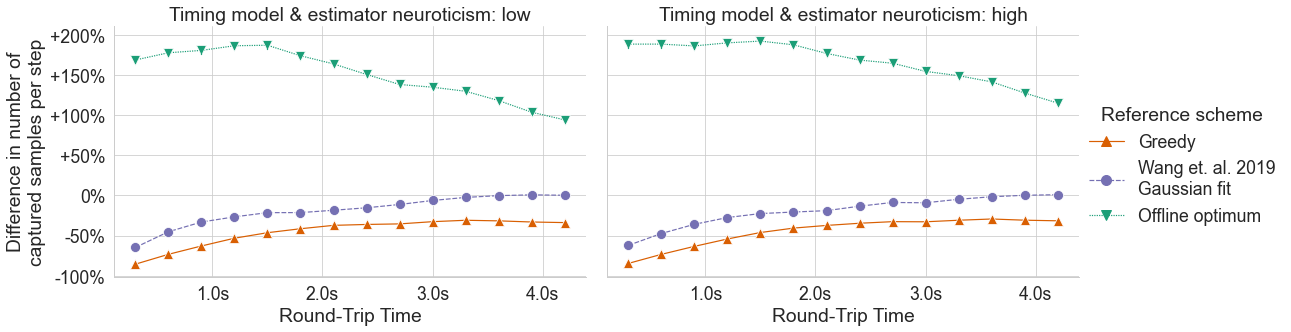
\includegraphics[width=\textwidth]{figs/new_model/sampling_optimization_diff.png}
        \caption{}
    \end{subfigure}
    \caption{Sampling optimization}
\end{figure*}

\begin{figure*}
    \centering
    \begin{subfigure}[t]{\textwidth}
        \centering
        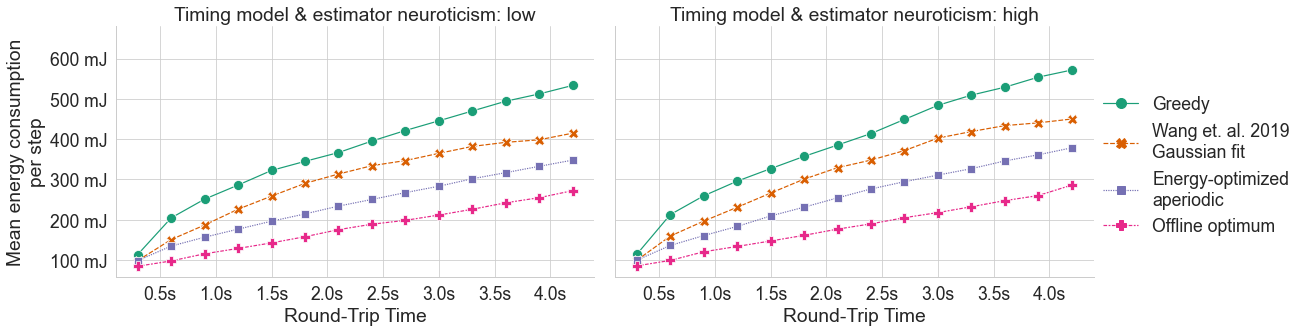
\includegraphics[width=\textwidth]{figs/new_model/energy_optimization.png}
        \caption{}
    \end{subfigure}\\
    \medskip
    \begin{subfigure}[t]{\textwidth}
        \centering
        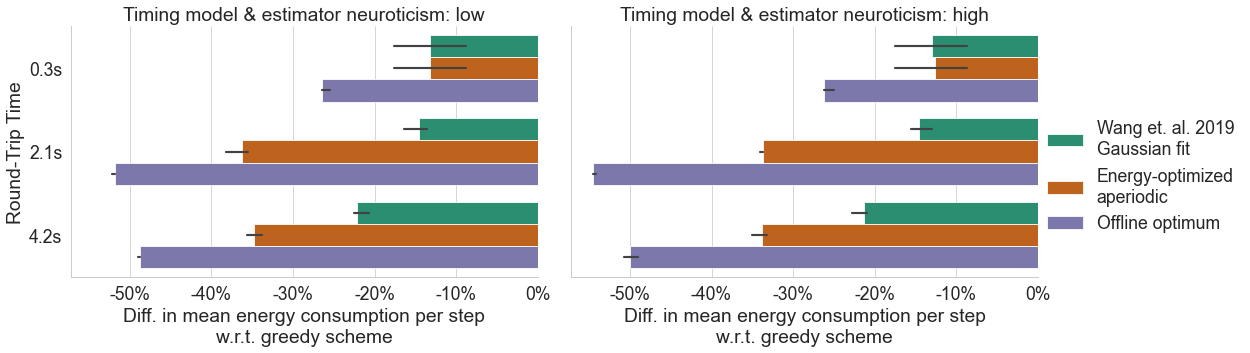
\includegraphics[width=\textwidth]{figs/new_model/energy_optimization_diff.png}
        \caption{}
    \end{subfigure}
    \caption{Energy optimization}
\end{figure*}